\documentclass[aspectratio=169]{beamer}

\usetheme{metropolis} % Use metropolis theme 

\usepackage{appendixnumberbeamer}
\usepackage{booktabs}

\usefonttheme[onlymath]{serif} 
\usepackage{mathpazo}
\usepackage{amsmath}
\usepackage{amsthm}

\title{Race in motion: sorting, segregation, colocation in Brazil}
\date{\today}
\author{Hyoungchul Kim (Wharton, UPenn)}

\begin{document}

\maketitle

\begin{frame}{Motivation}

	\begin{itemize}
		\item Socioeconomic inequality is closely linked to residential choice, both across and within cities (Moretti, 2013).
		\item As local amenities and productivities endogenously respond to the local population, this feedback loop could amplify inequality.
		\item One important socio-demographic when discussing location choice: \textbf{Race}.
		\item Important issue in both developed and developing country: racial segregation. 
		\item It is important to characterize factors affecting people's location preferences by race to fully understand the dynamics of residential patterns.
	\end{itemize}


\end{frame}

\begin{frame}{Research question (tentative)}
	\textbf{Some potential research questions}	
	\begin{enumerate}
		\item How do preference heterogeneity (by race) over amenities and productivity shape location sorting and inequality? 
		\item Quantify push- and pull- factors of people's location choices by race and its implications for local amenities and productivities in developing country setting.
		\item Develop a unified framework for across-city location choices w.r.t. productivity and amenities.
	\end{enumerate}
\end{frame}

\begin{frame}{(Brief) Literature review}
\begin{enumerate}
	\item Sorting across/within cities: \textcolor{gray}{Ahlfeldt et al. (2015); Diamond (2016); Sebastian et al. (2015); Ferreira and Wong (2023); Almagro and Dominguez (2025);.}\\
		$\Rightarrow$ Understand factors leading to sorting and colocation by race.\vspace{1em}
	\item Residential segregation: \textcolor{gray}{Wong (2013); Asher et al. (2024); Harari (2024).}\\
		$\Rightarrow$ Focus more on fully characterizing push- pull- \textbf{factors} leading to residential patterns by \textbf{race across} cities.\vspace{1em}

	\item Method-wise: \textcolor{gray}{Hsieh et al. (2019); Bryan and Morten (2019); Morten and Oliveira (2024)}
\end{enumerate}	
\end{frame}

\begin{frame}{Data}
\begin{enumerate}
	\item \textbf{Residential} Census microdata of Brazil (1970, 1980, 1991, 2000, 2010)
		\begin{itemize}
			\item Variable: \textbf{Race}, \textbf{Past locations}, socio-demographics.
		\end{itemize}\vspace{1em}
	\item \textbf{Workplace} RAIS data (formal sector employment; 1980 - 2023)
		\begin{itemize}
			\item Admin data on all formally employed workers across jobs in different industries and locations. 
		\end{itemize}\vspace{1em}
	\item \textbf{Workplace} ECINF data (informal sector employment; 2003) 
		\begin{itemize}
			\item Sample survey for self-employed workers in informal sector.
		\end{itemize}
\end{enumerate}	
\end{frame}

\begin{frame}{Research design: descriptive patterns about migration by race}

      \metroset{block=fill}

	\begin{alertblock}{Goal}
		Use location choice model by race to estimate relative migration attractiveness of Brazil municipalities \\ $\Rightarrow$ Show evidence of both colocation and separating force in play.
	\end{alertblock}

	\begin{block}{Motivation}
		\begin{itemize}
			\item Goal: Show variations and overlap of preferences of regions by race.
			\item It is hard to consider all factors that affect people's relative preferences for cities from scratch (Making restrictive assumptions).
			\item Reveal preference approach: observing where people move implicitly shows us their preferences without the need to fully characterize such factors upfront. 
			\item It also has additional benefits (e.g. Compared to surveys and population growth).
		\end{itemize}
	\end{block}
\end{frame}

\begin{frame}{Location choice setup}
	Following Lee, Lee and Lin (2021); Kim, Lee and Park (2023): \vspace{1em}

	\textbf{Environment setup}
	\begin{itemize}
		\item $J$ number of regions with initial populations. 
		\item Each region offers multiple opportunities ($k$) to a person with number increasing with population (\# of houses, jobs, etc). 
		\item (Individual) $\max_k U_{odk} = \overbrace{u_d}^{\text{\hidewidth Destination utility \hidewidth}} - \underbrace{c_{od}}_{\text{\hidewidth Migration cost \hidewidth}} + X + \varepsilon_{odk}$.
		\item \textcolor{red}{Note 1}: \# of opportunity generally increase with size of region.
		\item \textcolor{red}{Note 2}: Stayers are assumed to have chosen the region they are currently in.
	\end{itemize}
\end{frame}

\begin{frame}{Location choice setup}
	\textbf{Choice probability of choosing region $d$}	
	\begin{align}
		\pi_{od} = \frac{N_d^\gamma \exp(u_d - c_{od})}{\sum_j N_j^\gamma \exp(u_j - c_{oj})}\Rightarrow \frac{\exp(\delta_d - \log(d_{od})\beta)}{\sum_j \exp(\delta_j - \log\left(d_{od}  \right)\beta )}
	\end{align}

	\begin{itemize}
		\item $N_d^\gamma$ is the total \#  of opportunities offered by each city.
		\item $\gamma$ is a parameter that sets the relation between city size and number of opportunities.
		\item Parametric assumption: $\delta_d = \overbrace{Z_d' \alpha}^{\text{\hidewidth City characteristics \hidewidth}} + \gamma N_d \Rightarrow u_d = \delta_d - \gamma N_d $. 
		\item $Z_d' \alpha$ is linear unbiased predictor of city's welfare levels.
	\end{itemize}
\end{frame}

\begin{frame}{Example results}
	\begin{columns}
	\begin{column}{0.5\textwidth}
	\begin{figure}
		\resizebox{\textwidth}{!}{
		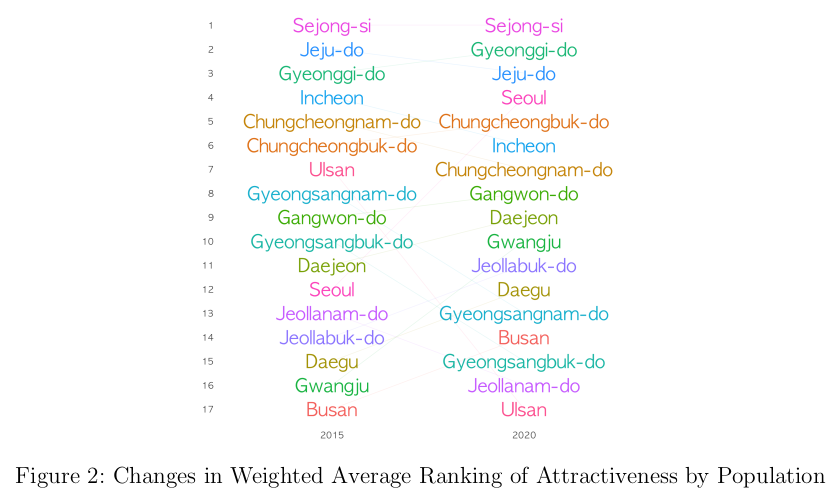
\includegraphics{ranking-year.png}

		}
	\end{figure}	
\end{column}
\begin{column}{0.5\textwidth}
	\begin{figure}
		\resizebox{\textwidth}{!}{
		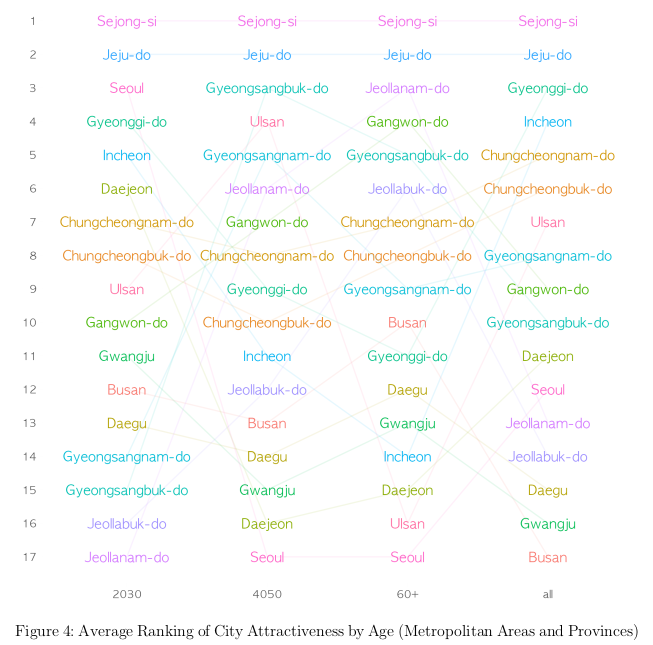
\includegraphics{ranking-age.png}

		}
	\end{figure}		
\end{column}
\end{columns}
\end{frame}

\begin{frame}{Possible results (hopefully)}
	\begin{itemize}
		\item Hopefully, there will be some variations and some correlations in people's ranking of cities by race.
		\item \textbf{Variations}: implies that there can be some homophily and/or segregation effects happening between race.
		\item \textbf{Correlations}: implies that there is also some preferences for certain types of people with different ethical backgrounds to be close to each other.
		\item Nice way to visualize some possible effects happening and a starting point for some full model to characterize possible mechanisms.
	\end{itemize}
\end{frame}

\begin{frame}{Research design: economic model}
	\textbf{Why do we need a model?}	
	\begin{itemize}
		\item GE effects: our previous results assume partial eqm.
		\item Integration of differential and overlapping patterns of people by race.
		\item Dynamics!
		\item Deep parameters of interest: e.g. (dis)-utility from density. 
		\item Setup a full unified framework that captures this migration sorting and eqm effects.
	\end{itemize}
\end{frame}

\begin{frame}{(Preliminary) Economic model: key building blocks}
	\textbf{Environment setup}	
	\begin{itemize}
		\item Individuals $i$ indexed by their race type $r \in R$. $N_r$ is total number of individuals of race $r$. 
		\item Individuals consume goods and housing accord with a C-D utility function.
		\item Individuals also enjoy amenity $B_{dt}$ of living in location $d$.
		\item Given this indirect utility, individual living in origin $o$ will choose which destination $d$ to live in (migration cost $c_{odt}$). iid shock for each destination.
		\item Each location can use labor to produce goods (productivity draw)\ldots
	\end{itemize}

	I am looking into literature to think more about the model setup.
\end{frame}

\begin{frame}{Conclusion \& Next steps}
	\begin{enumerate}
		\item Apply to get access to necessary data.
		\item First do some descriptive analysis I mentioned in the slide to see overall patterns.
		\item If previous steps look promising, start focusing bit more about the model.
	\end{enumerate}	
\end{frame}

\end{document}
